\documentclass{ximera}  


%\usepackage{todonotes}
%\usepackage{mathtools} %% Required for wide table Curl and Greens
%\usepackage{cuted} %% Required for wide table Curl and Greens
\newcommand{\todo}{}

\usepackage{esint} % for \oiint
\ifxake%%https://math.meta.stackexchange.com/questions/9973/how-do-you-render-a-closed-surface-double-integral
\renewcommand{\oiint}{{\large\bigcirc}\kern-1.56em\iint}
\fi


\graphicspath{
  {./}
  {jpg}
  {ximeraTutorial/}
  {basicPhilosophy/}
  {functionsOfSeveralVariables/}
  {normalVectors/}
  {lagrangeMultipliers/}
  {vectorFields/}
  {greensTheorem/}
  {shapeOfThingsToCome/}
  {dotProducts/}
  {partialDerivativesAndTheGradientVector/}
  {../productAndQuotientRules/exercises/}
  {../motionAndPathsInSpace/exercises/}
  {../normalVectors/exercisesParametricPlots/}
  {../continuityOfFunctionsOfSeveralVariables/exercises/}
  {../partialDerivativesAndTheGradientVector/exercises/}
  {../directionalDerivativeAndChainRule/exercises/}
  {../commonCoordinates/exercisesCylindricalCoordinates/}
  {../commonCoordinates/exercisesSphericalCoordinates/}
  {../greensTheorem/exercisesCurlAndLineIntegrals/}
  {../greensTheorem/exercisesDivergenceAndLineIntegrals/}
  {../shapeOfThingsToCome/exercisesDivergenceTheorem/}
  {../greensTheorem/}
  {../shapeOfThingsToCome/}
  {../separableDifferentialEquations/exercises/}
  {vectorFields/}
}

\newcommand{\mooculus}{\textsf{\textbf{MOOC}\textnormal{\textsf{ULUS}}}}

\usepackage{tkz-euclide}\usepackage{tikz}
\usepackage{tikz-cd}
\usetikzlibrary{arrows}
\tikzset{>=stealth,commutative diagrams/.cd,
  arrow style=tikz,diagrams={>=stealth}} %% cool arrow head
\tikzset{shorten <>/.style={ shorten >=#1, shorten <=#1 } } %% allows shorter vectors

\usetikzlibrary{backgrounds} %% for boxes around graphs
\usetikzlibrary{shapes,positioning}  %% Clouds and stars
\usetikzlibrary{matrix} %% for matrix
\usepgfplotslibrary{polar} %% for polar plots
\usepgfplotslibrary{fillbetween} %% to shade area between curves in TikZ
\usetkzobj{all}
\usepackage[makeroom]{cancel} %% for strike outs
%\usepackage{mathtools} %% for pretty underbrace % Breaks Ximera
%\usepackage{multicol}
\usepackage{pgffor} %% required for integral for loops



%% http://tex.stackexchange.com/questions/66490/drawing-a-tikz-arc-specifying-the-center
%% Draws beach ball
\tikzset{pics/carc/.style args={#1:#2:#3}{code={\draw[pic actions] (#1:#3) arc(#1:#2:#3);}}}



\usepackage{array}
\setlength{\extrarowheight}{+.1cm}
\newdimen\digitwidth
\settowidth\digitwidth{9}
\def\divrule#1#2{
\noalign{\moveright#1\digitwidth
\vbox{\hrule width#2\digitwidth}}}





\newcommand{\RR}{\mathbb R}
\newcommand{\R}{\mathbb R}
\newcommand{\N}{\mathbb N}
\newcommand{\Z}{\mathbb Z}

\newcommand{\sagemath}{\textsf{SageMath}}


%\renewcommand{\d}{\,d\!}
\renewcommand{\d}{\mathop{}\!d}
\newcommand{\dd}[2][]{\frac{\d #1}{\d #2}}
\newcommand{\pp}[2][]{\frac{\partial #1}{\partial #2}}
\renewcommand{\l}{\ell}
\newcommand{\ddx}{\frac{d}{\d x}}

\newcommand{\zeroOverZero}{\ensuremath{\boldsymbol{\tfrac{0}{0}}}}
\newcommand{\inftyOverInfty}{\ensuremath{\boldsymbol{\tfrac{\infty}{\infty}}}}
\newcommand{\zeroOverInfty}{\ensuremath{\boldsymbol{\tfrac{0}{\infty}}}}
\newcommand{\zeroTimesInfty}{\ensuremath{\small\boldsymbol{0\cdot \infty}}}
\newcommand{\inftyMinusInfty}{\ensuremath{\small\boldsymbol{\infty - \infty}}}
\newcommand{\oneToInfty}{\ensuremath{\boldsymbol{1^\infty}}}
\newcommand{\zeroToZero}{\ensuremath{\boldsymbol{0^0}}}
\newcommand{\inftyToZero}{\ensuremath{\boldsymbol{\infty^0}}}



\newcommand{\numOverZero}{\ensuremath{\boldsymbol{\tfrac{\#}{0}}}}
\newcommand{\dfn}{\textbf}
%\newcommand{\unit}{\,\mathrm}
\newcommand{\unit}{\mathop{}\!\mathrm}
\newcommand{\eval}[1]{\bigg[ #1 \bigg]}
\newcommand{\seq}[1]{\left( #1 \right)}
\renewcommand{\epsilon}{\varepsilon}
\renewcommand{\phi}{\varphi}


\renewcommand{\iff}{\Leftrightarrow}

\DeclareMathOperator{\arccot}{arccot}
\DeclareMathOperator{\arcsec}{arcsec}
\DeclareMathOperator{\arccsc}{arccsc}
\DeclareMathOperator{\si}{Si}
\DeclareMathOperator{\scal}{scal}
\DeclareMathOperator{\sign}{sign}


%% \newcommand{\tightoverset}[2]{% for arrow vec
%%   \mathop{#2}\limits^{\vbox to -.5ex{\kern-0.75ex\hbox{$#1$}\vss}}}
\newcommand{\arrowvec}[1]{{\overset{\rightharpoonup}{#1}}}
%\renewcommand{\vec}[1]{\arrowvec{\mathbf{#1}}}
\renewcommand{\vec}[1]{{\overset{\boldsymbol{\rightharpoonup}}{\mathbf{#1}}}\hspace{0in}}

\newcommand{\point}[1]{\left(#1\right)} %this allows \vector{ to be changed to \vector{ with a quick find and replace
\newcommand{\pt}[1]{\mathbf{#1}} %this allows \vec{ to be changed to \vec{ with a quick find and replace
\newcommand{\Lim}[2]{\lim_{\point{#1} \to \point{#2}}} %Bart, I changed this to point since I want to use it.  It runs through both of the exercise and exerciseE files in limits section, which is why it was in each document to start with.

\DeclareMathOperator{\proj}{\mathbf{proj}}
\newcommand{\veci}{{\boldsymbol{\hat{\imath}}}}
\newcommand{\vecj}{{\boldsymbol{\hat{\jmath}}}}
\newcommand{\veck}{{\boldsymbol{\hat{k}}}}
\newcommand{\vecl}{\vec{\boldsymbol{\l}}}
\newcommand{\uvec}[1]{\mathbf{\hat{#1}}}
\newcommand{\utan}{\mathbf{\hat{t}}}
\newcommand{\unormal}{\mathbf{\hat{n}}}
\newcommand{\ubinormal}{\mathbf{\hat{b}}}

\newcommand{\dotp}{\bullet}
\newcommand{\cross}{\boldsymbol\times}
\newcommand{\grad}{\boldsymbol\nabla}
\newcommand{\divergence}{\grad\dotp}
\newcommand{\curl}{\grad\cross}
%\DeclareMathOperator{\divergence}{divergence}
%\DeclareMathOperator{\curl}[1]{\grad\cross #1}
\newcommand{\lto}{\mathop{\longrightarrow\,}\limits}

\renewcommand{\bar}{\overline}

\colorlet{textColor}{black}
\colorlet{background}{white}
\colorlet{penColor}{blue!50!black} % Color of a curve in a plot
\colorlet{penColor2}{red!50!black}% Color of a curve in a plot
\colorlet{penColor3}{red!50!blue} % Color of a curve in a plot
\colorlet{penColor4}{green!50!black} % Color of a curve in a plot
\colorlet{penColor5}{orange!80!black} % Color of a curve in a plot
\colorlet{penColor6}{yellow!70!black} % Color of a curve in a plot
\colorlet{fill1}{penColor!20} % Color of fill in a plot
\colorlet{fill2}{penColor2!20} % Color of fill in a plot
\colorlet{fillp}{fill1} % Color of positive area
\colorlet{filln}{penColor2!20} % Color of negative area
\colorlet{fill3}{penColor3!20} % Fill
\colorlet{fill4}{penColor4!20} % Fill
\colorlet{fill5}{penColor5!20} % Fill
\colorlet{gridColor}{gray!50} % Color of grid in a plot

\newcommand{\surfaceColor}{violet}
\newcommand{\surfaceColorTwo}{redyellow}
\newcommand{\sliceColor}{greenyellow}




\pgfmathdeclarefunction{gauss}{2}{% gives gaussian
  \pgfmathparse{1/(#2*sqrt(2*pi))*exp(-((x-#1)^2)/(2*#2^2))}%
}


%%%%%%%%%%%%%
%% Vectors
%%%%%%%%%%%%%

%% Simple horiz vectors
\renewcommand{\vector}[1]{\left\langle #1\right\rangle}


%% %% Complex Horiz Vectors with angle brackets
%% \makeatletter
%% \renewcommand{\vector}[2][ , ]{\left\langle%
%%   \def\nextitem{\def\nextitem{#1}}%
%%   \@for \el:=#2\do{\nextitem\el}\right\rangle%
%% }
%% \makeatother

%% %% Vertical Vectors
%% \def\vector#1{\begin{bmatrix}\vecListA#1,,\end{bmatrix}}
%% \def\vecListA#1,{\if,#1,\else #1\cr \expandafter \vecListA \fi}

%%%%%%%%%%%%%
%% End of vectors
%%%%%%%%%%%%%

%\newcommand{\fullwidth}{}
%\newcommand{\normalwidth}{}



%% makes a snazzy t-chart for evaluating functions
%\newenvironment{tchart}{\rowcolors{2}{}{background!90!textColor}\array}{\endarray}

%%This is to help with formatting on future title pages.
\newenvironment{sectionOutcomes}{}{}



%% Flowchart stuff
%\tikzstyle{startstop} = [rectangle, rounded corners, minimum width=3cm, minimum height=1cm,text centered, draw=black]
%\tikzstyle{question} = [rectangle, minimum width=3cm, minimum height=1cm, text centered, draw=black]
%\tikzstyle{decision} = [trapezium, trapezium left angle=70, trapezium right angle=110, minimum width=3cm, minimum height=1cm, text centered, draw=black]
%\tikzstyle{question} = [rectangle, rounded corners, minimum width=3cm, minimum height=1cm,text centered, draw=black]
%\tikzstyle{process} = [rectangle, minimum width=3cm, minimum height=1cm, text centered, draw=black]
%\tikzstyle{decision} = [trapezium, trapezium left angle=70, trapezium right angle=110, minimum width=3cm, minimum height=1cm, text centered, draw=black]




 
\title{Transmission-line impedance matching} 
\author{Milica Markovic} 
\outcome{Design a transmission-line impedance matching network for any load impedance and discuss pros and cons of various designs.}
\begin{document}  
\begin{abstract}  

\end{abstract}  
\maketitle    



\section{Design of a transmission-line impedance matching circuits}

Transmission-line impedance matching circuits are used at higher frequencies where the lumped elements become very small and impractical to use. 

To design fully transmission-line matching circuits, we have to first learn how to replace the lumped element in the matching circuit from the last step in the previous section with a transmission line. 

\subsection{Replacing lumped-elements with equivalent transmission-line stubs}

To make fully transmission line impedance matching circuits, we can replace capacitors and inductors with ``stubs", which are shorted or open transmission lines. 

The input impedance of shorted or open transmission lines can be made purely inductive or capacitive, as shown in Figures \ref{fig:OpenStubLambdaOver8}-\ref{fig:ShortedStubLambdaOver8}. SWR circle of an open or shorted stub is the outer perimeter of the Smith Chart. The length of the transmission line will determine the input impedance of the stub. The input impedance is always purely reactive. 


To gain intuition of how the input impedance changes, as the length of the line changes, for a transmission-line terminated in open circuit, use the following simulation. In the simulation, change the length of the line, and observe how the input impedance changes.

\begin{center}  
\geogebra{w5fkzhvj}{800}{600}  
\end{center} 

\begin{example}

Find the input impedance of a $\frac{\lambda}{8}$ long transmission line terminated in an open circuit.

\begin{explanation}

In Figure \ref{fig:OpenStubLambdaOver8}, the length of the line is  $\frac{\lambda}{8}$. The ``load" connected to the output of this line is an open circuit $Z_L=\infty$. 


On the Smith Chart, we start from the load impedance and add a $0.125 \lambda$ line, following the WTG scale. The input impedance is purely capacitive $Z_{in}=-j$. 

\begin{figure}[htbp]
\begin{center}
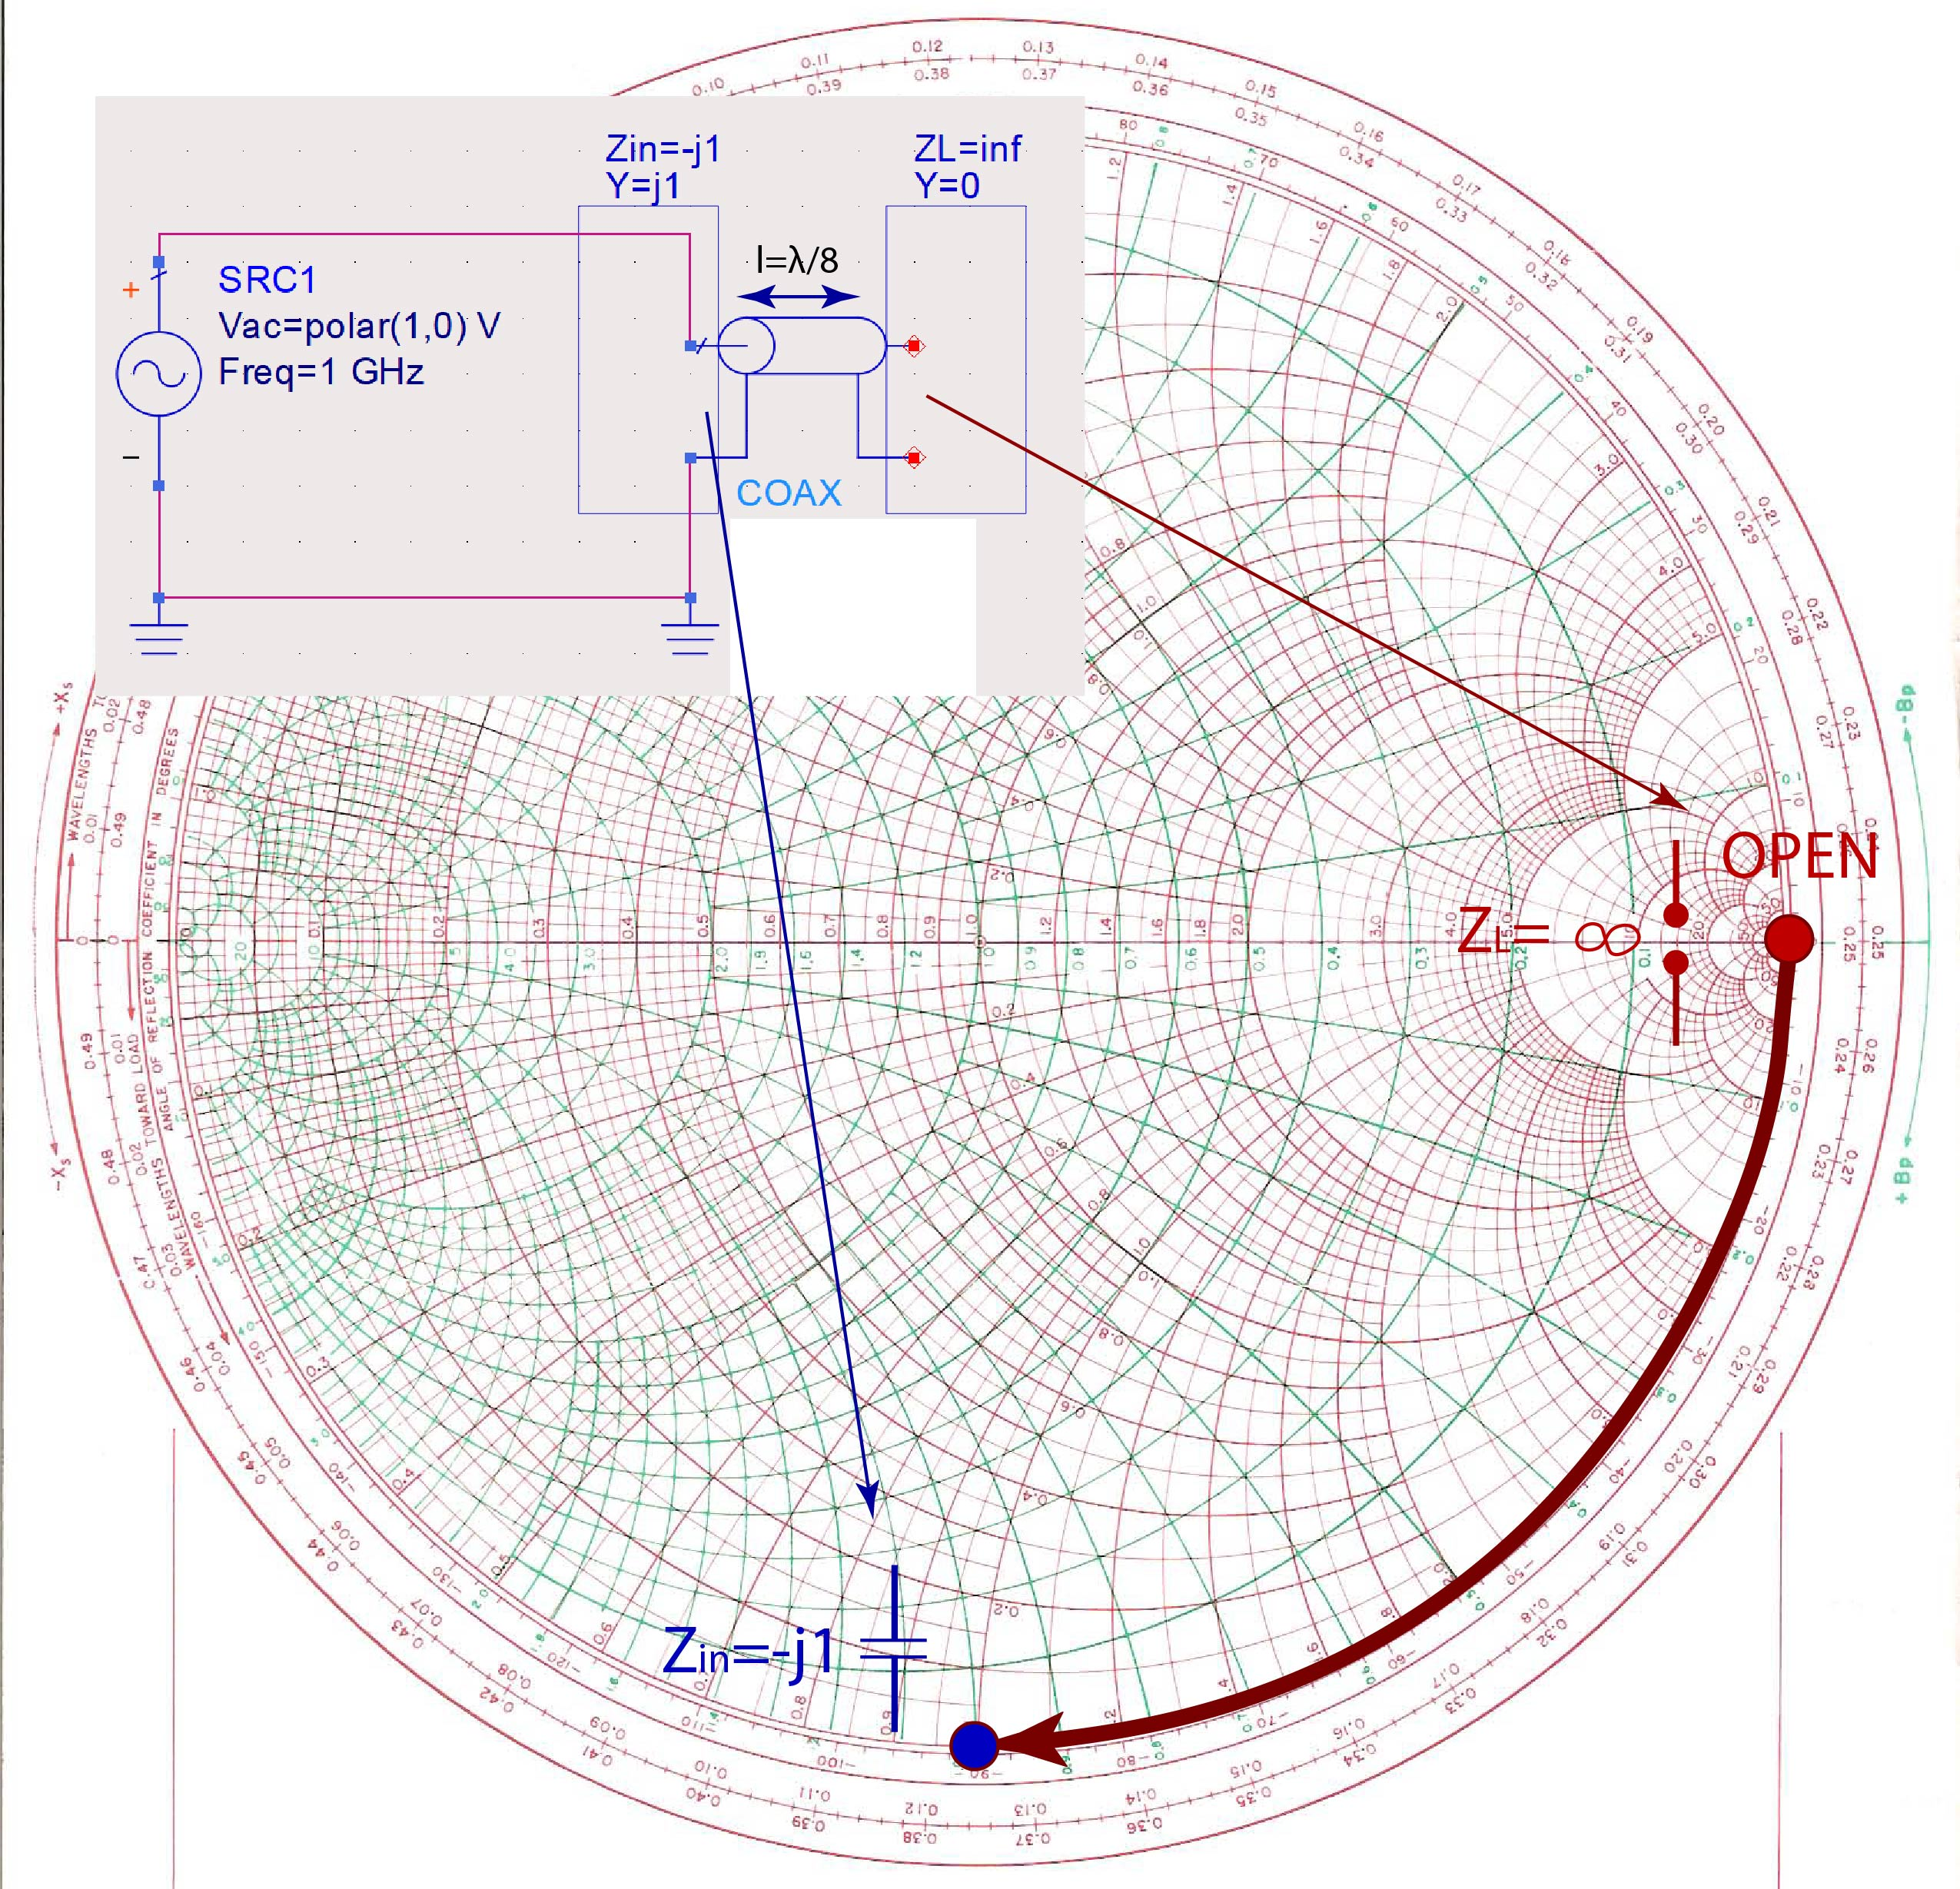
\includegraphics[scale=0.87]{../jpg/openstub-01.jpg}
\end{center}
\caption{Input impedance $Z_{in}=-j$ of a $\frac{\lambda}{8}$ open transmission line.}
\label{fig:OpenStubLambdaOver8}
\end{figure}

The input impedance is equal to a capacitor's impedance $Z_{in}=-j$ at a single frequency, where the electrical length of the line is $0.125 \lambda$. At other frequencies, the electrical length of the line is different, and therefore the input impedance is lower or higher than $Z_{in}=-j$.

\end{explanation}
\end{example}



\begin{example}

Find the input impedance of a $\frac{3 \lambda}{8}$ long transmission line terminated in an open circuit.


\begin{explanation}

Another example is shown in Figure \ref{fig:OpenStub3LambdaOver8}, where the length of the line is  $\frac{3 \lambda}{8}$. The load connected to this line is again an open circuit $Z_L=\infty$. On the Smith Chart, we start from the load impedance and add a $0.375 \lambda$ line, following the WTG scale. The input impedance is purely inductive $Z_{in}=j$.

\begin{figure}[htbp]
\begin{center}
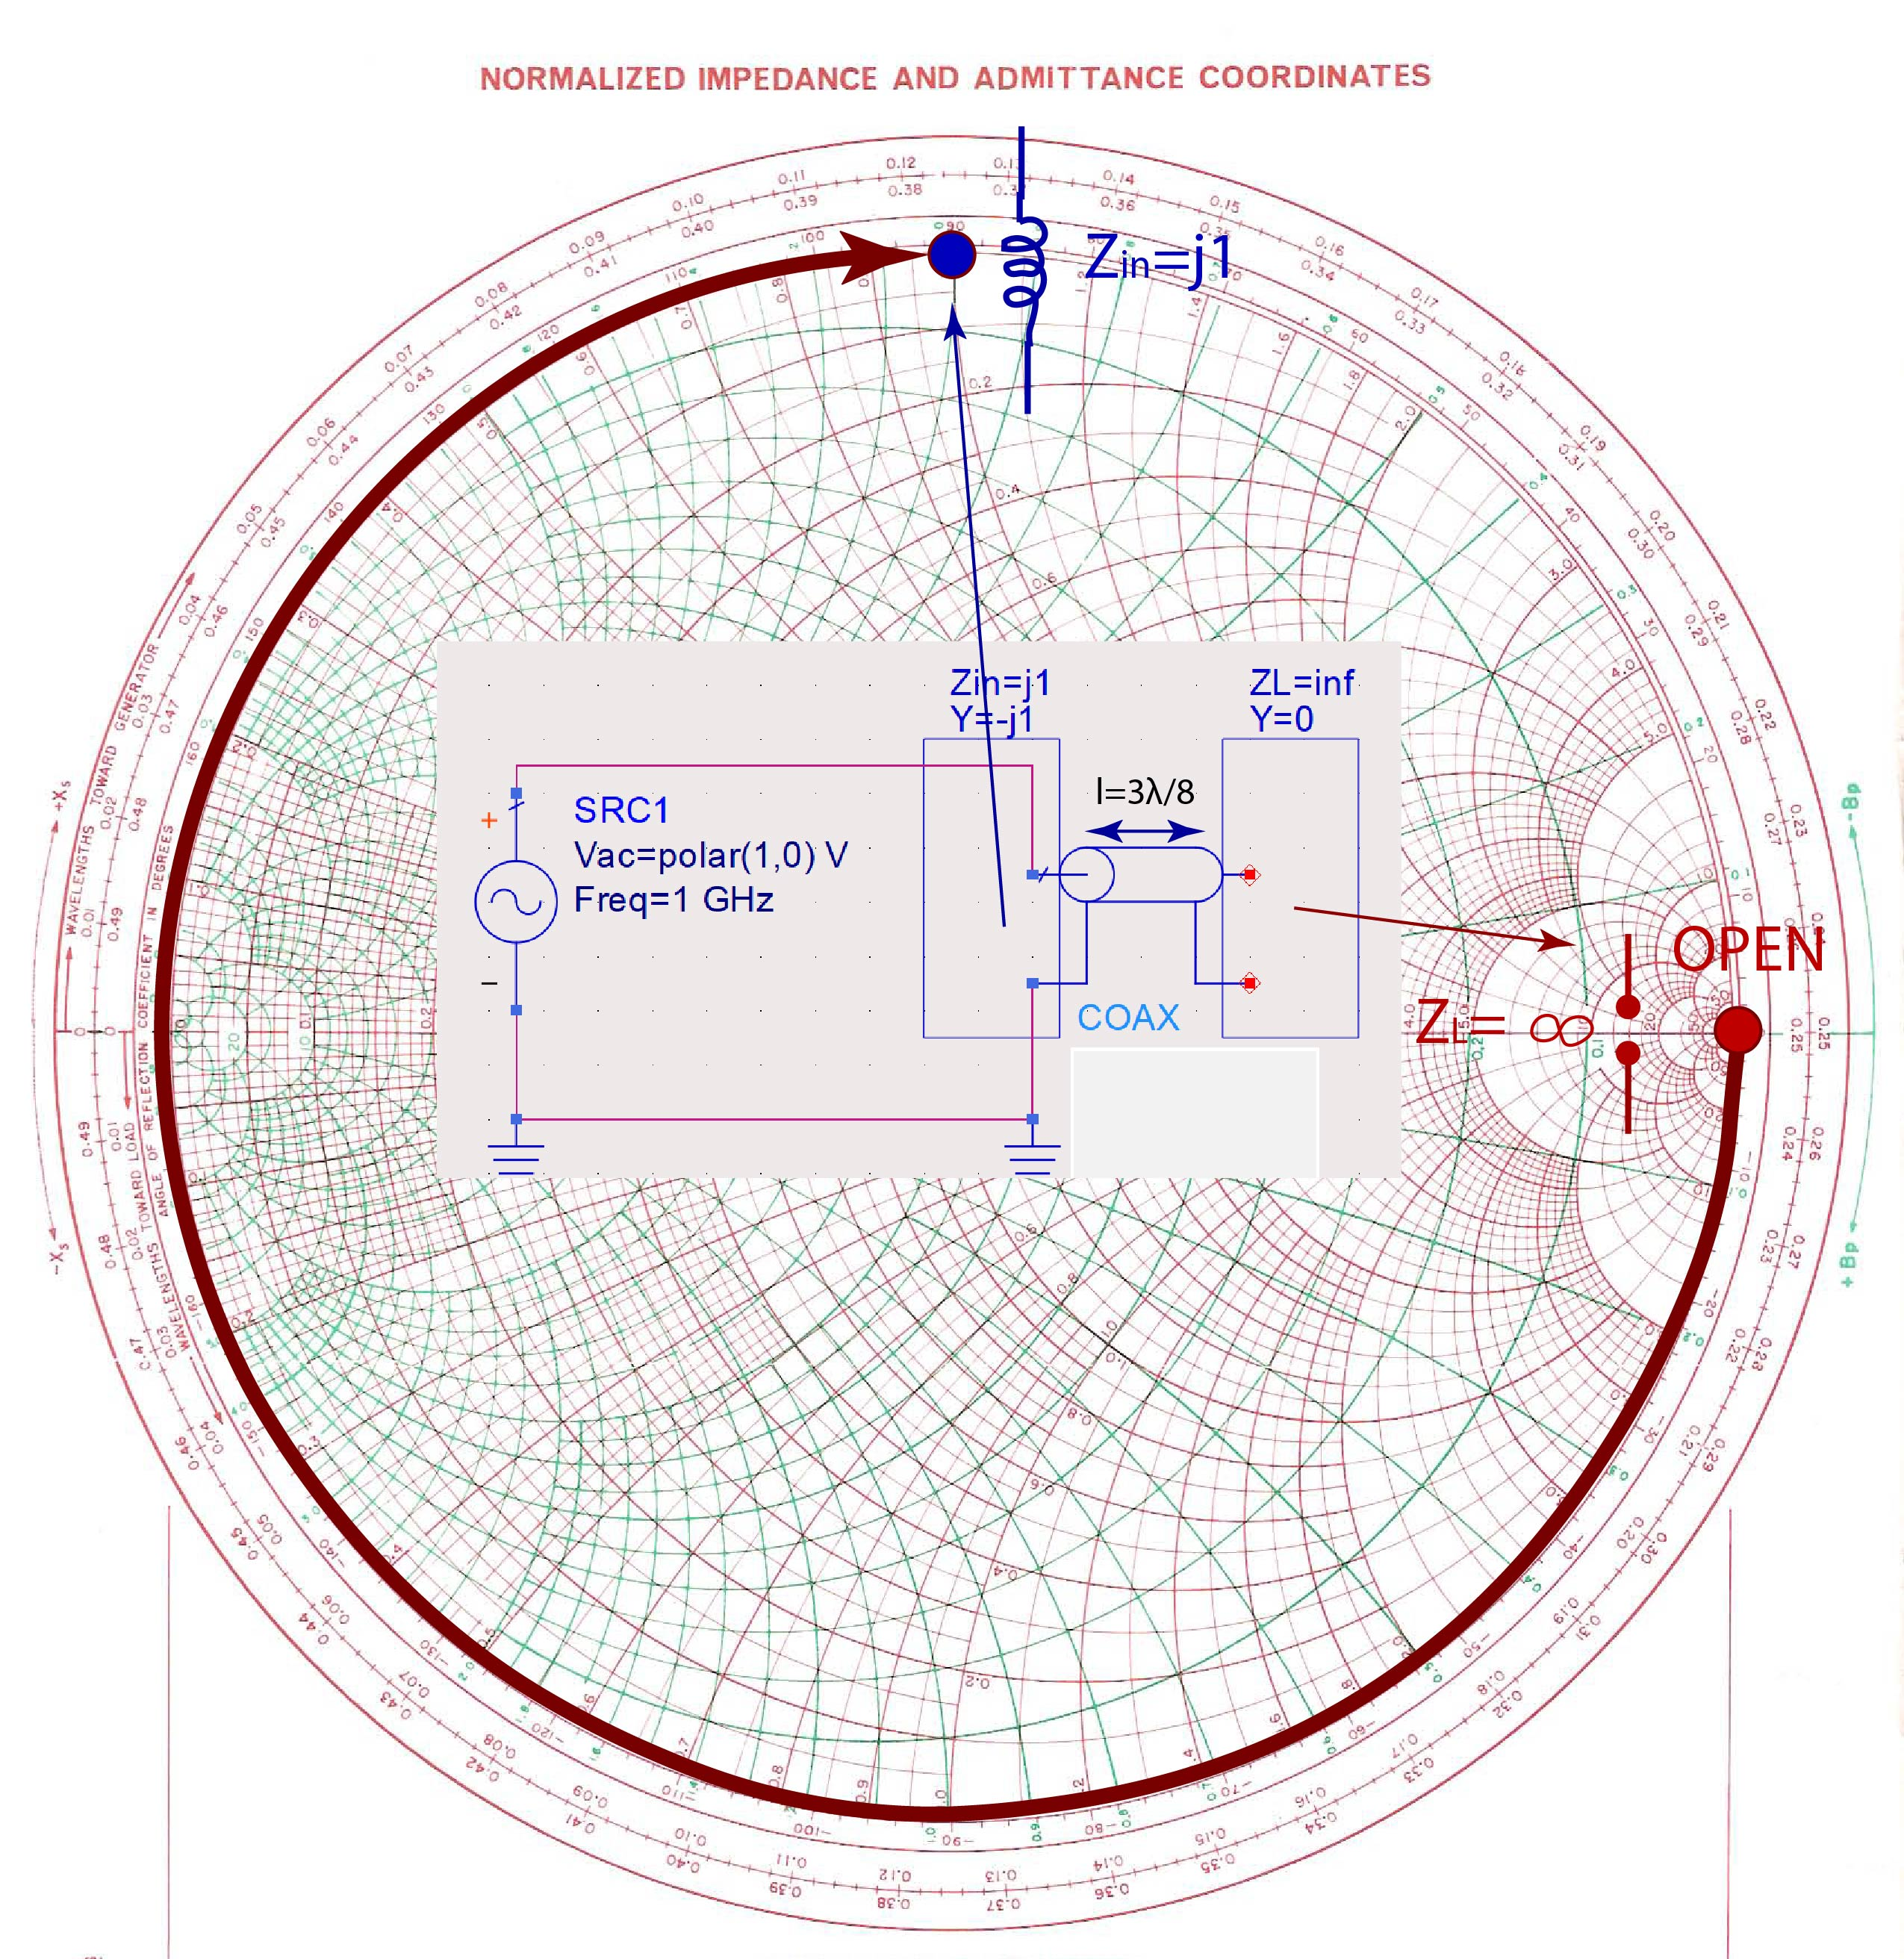
\includegraphics[scale=1]{../jpg/openstub2-01.jpg}
\end{center}
\caption{Input impedance $Z_{in}=j$  of a $\frac{3 \lambda}{8}$ open transmission line.}
\label{fig:OpenStub3LambdaOver8}
\end{figure}


\end{explanation}
\end{example}

\subsubsection{Simulation of the input impedance of shorted stub}

So far we discussed the open circuit at the end of the line. To see how input impedance the input impedance changes, as the length of the line changes, for a transmission-line terminated in a {\bf short} circuit, use the following simulation. In the simulation, change the length of the line, and observe how the input impedance changes. How is this case different than the previous one?

\begin{center}  
\geogebra{yutfjed9}{800}{600}  
\end{center} 


\begin{example}


Find the input impedance of a $\frac{\lambda}{8}$ long transmission line terminated in a short circuit.

\begin{explanation}
The last example is shown in Figure \ref{fig:ShortedStubLambdaOver8}, where the length of the line is  $\frac{3 \lambda}{8}$. The load connected to this line is now a short circuit $Z_L=0 \Omega$. On the Smith Chart, we start from the load impedance and add a $0.375 \lambda$ line, following the WTG scale. The input impedance is purely inductive $Z_{in}=j$.



\begin{figure}[htbp]
\begin{center}
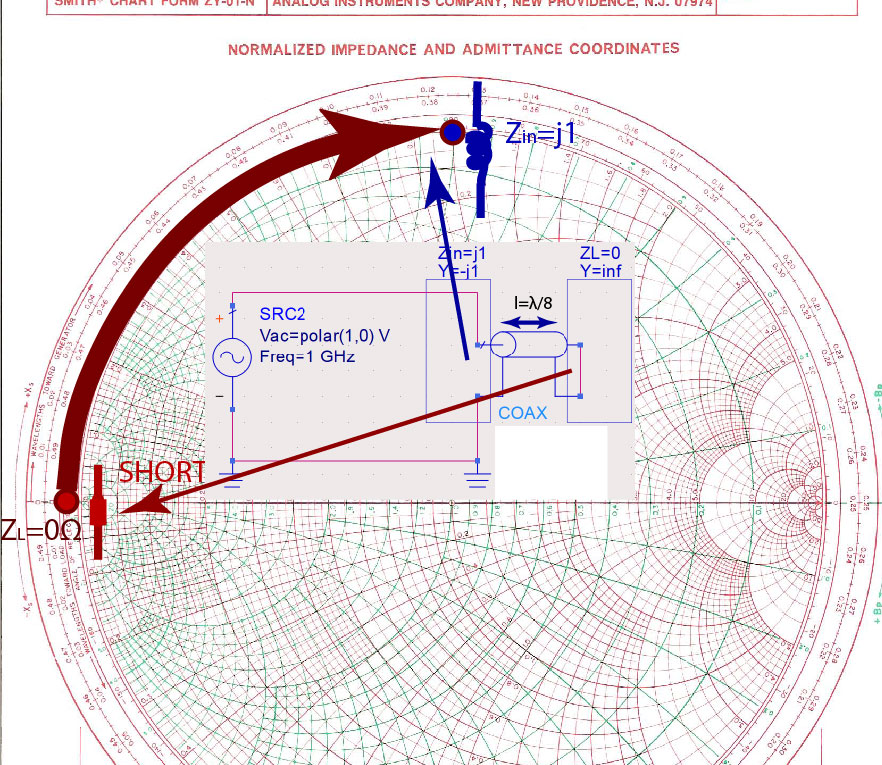
\includegraphics[scale=1]{../jpg/shortedstub-01.jpg}
\end{center}
\caption{Input impedance $Z_{in}=j$ of a $\frac{\lambda}{8}$ shorted transmission line.}
\label{fig:ShortedStubLambdaOver8}
\end{figure}



\end{explanation}
\end{example}

\newpage


\subsection{Fully transmission-line matching circuits.}

The first few steps in the fully transmission-line matching circuit are the same as in the mixed-impedance matching. We find the point on the Smith Chart that represents the normalized impedance of the load $Z_L=0.5+j1$, as in Figure \ref{fig:NormImponSC}. 

\begin{figure}[htbp]
\begin{center}
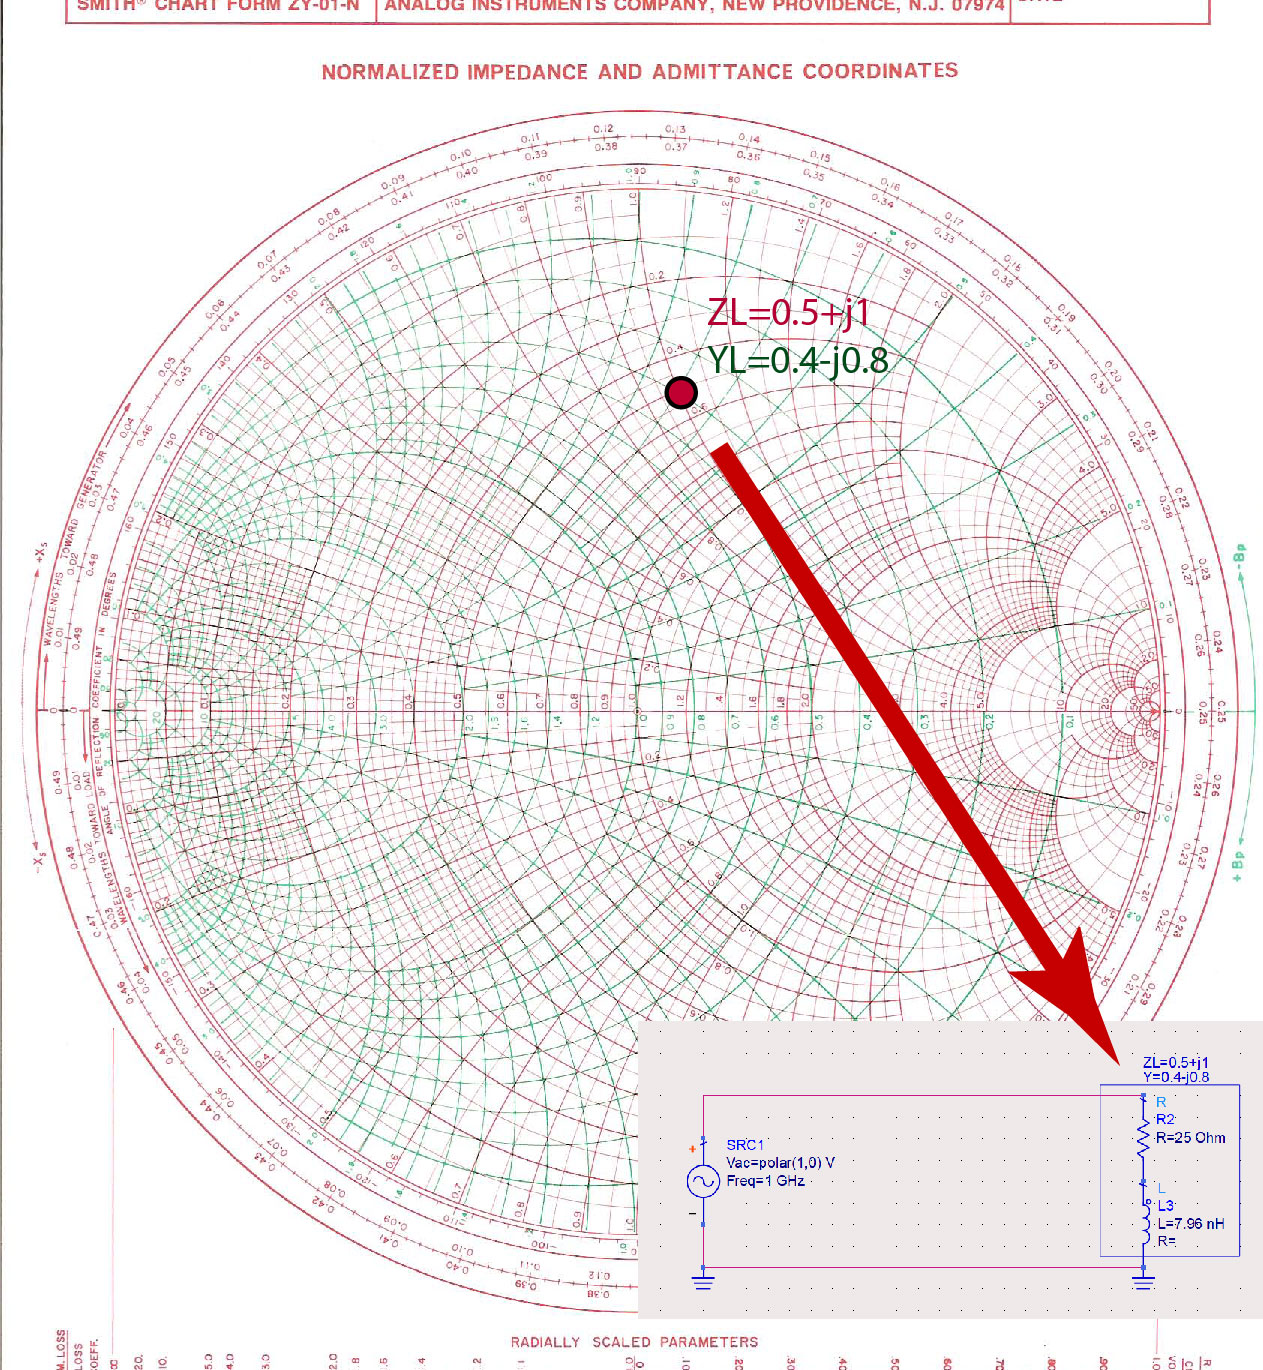
\includegraphics[scale=1]{../jpg/MixedMatch2-01.jpg}
\end{center}
\caption{Position of normalized impedance $Z_L=0.5+j1$ on Smith Chart.}
\label{fig:NormImponSC}
\end{figure}

A section of transmission line has to be added to impedance $Z_L=0.5+j1$ to transform the load impedance to input admittance $Y_{in}=1+1.6$, as shown in Figure \ref{fig:AddingSectionOfLine}. The length of the line is calculated by reading the position of the load impedance and input impedance on the WTG circle. Load impedance is at $0.135 \lambda$, and the input impedance is at $0.425 \lambda$. The difference between these two positions gives us the length of the line $0.29 \lambda$. In electrical degrees, this length is approximately $105^0$. The input admittance to the line is now $Y_L=1+1.6$. 


\begin{figure}[htbp]
\begin{center}
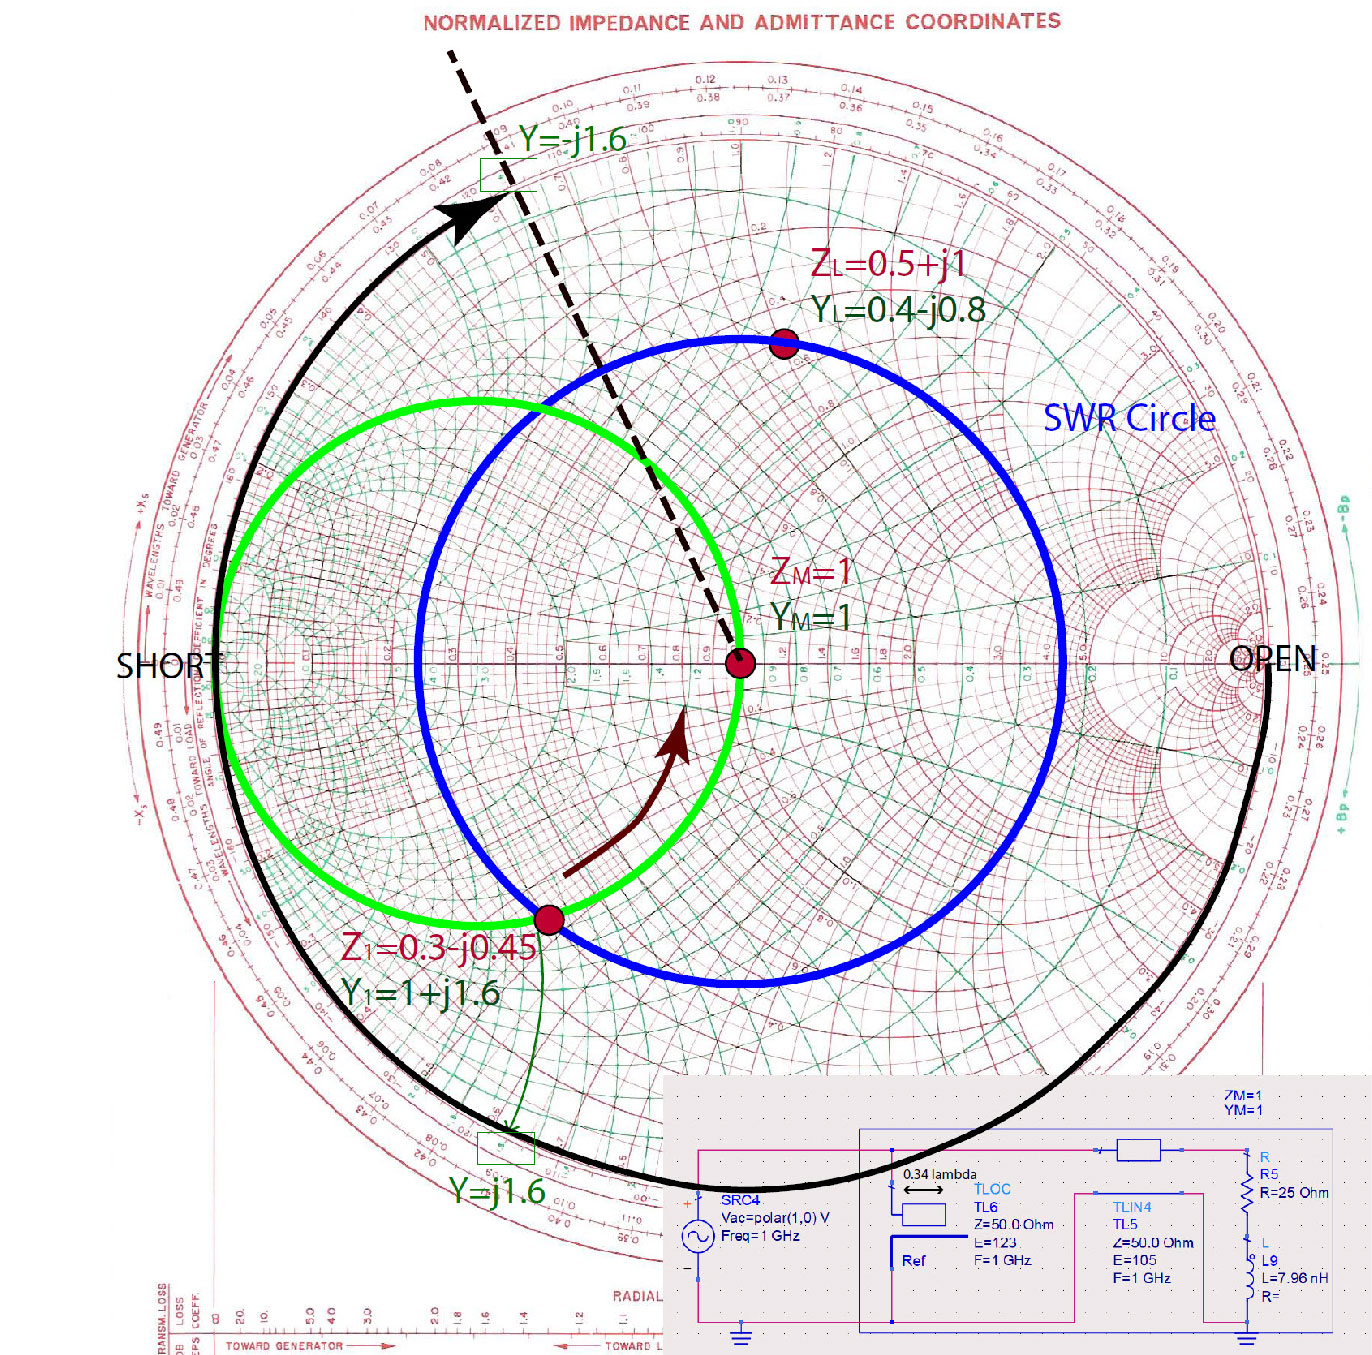
\includegraphics[scale=1]{../jpg/MatchTL-01.jpg}
\end{center}
\caption{The result of impedance matching.}
\label{fig:AddingSectionOfLine}
\end{figure}

The last step is to determine the shunt reactance that will remove the reactive part of the admittance $Y_L=1+1.6$, and make the total input impedance and admittance $Z_M=Y_M=1$. By inspection, we have to add $Y_{add}=-j1.6$. A lumped element in parallel (because we are adding two admittances), as in the previous mixed-matching problem, is an inductor (because admittance of an inductor is negative)  $Y_{add}=\frac{1}{j \omega L}=-j1.6$. However, we want to make a fully transmission line impedance matching circuit. Therefore, we have to replace the inductor with an equivalent transmission line, a stub. 

We can pick whether the stub is open or shorted. Usually, we want to pick the shortest possible stub, because the smaller the stub, the smaller the circuit will be. In some other cases, it is easier to leave the transmission line open, because making a short circuit requires drilling the PC Board and making a via-hole to connect the line to the ground. In this case, we picked an open stub to replace the lumped element, as shown in Figure \ref{fig:TransLineImpM}.

To find the stub that will have the same input admittance as an inductor $Y_{add}=-j1.6$, we first identify the position of admittance $-j1.6$ on the Smith Chart. This is the input impedance of the stub. We picked an open circuit for the load of the stub. To find the length of the stub, we start on the position of WTG scale from the load $Z_L=\infty$, WTG=$0.25 \lambda$, going in the WTG direction, we pass the short circuit position WTG=$0$, and then another WTG=$0.09 \lambda$ to reach the input admittance of $-j1.6$. The length of the stub is $0.25 \lambda+0.09 \lambda=0.34 \lambda$. In electrical degrees, this length is $\Theta=\beta l =2 \pi 0.34 \approx 123^0$.




\begin{figure}[htbp]
\begin{center}
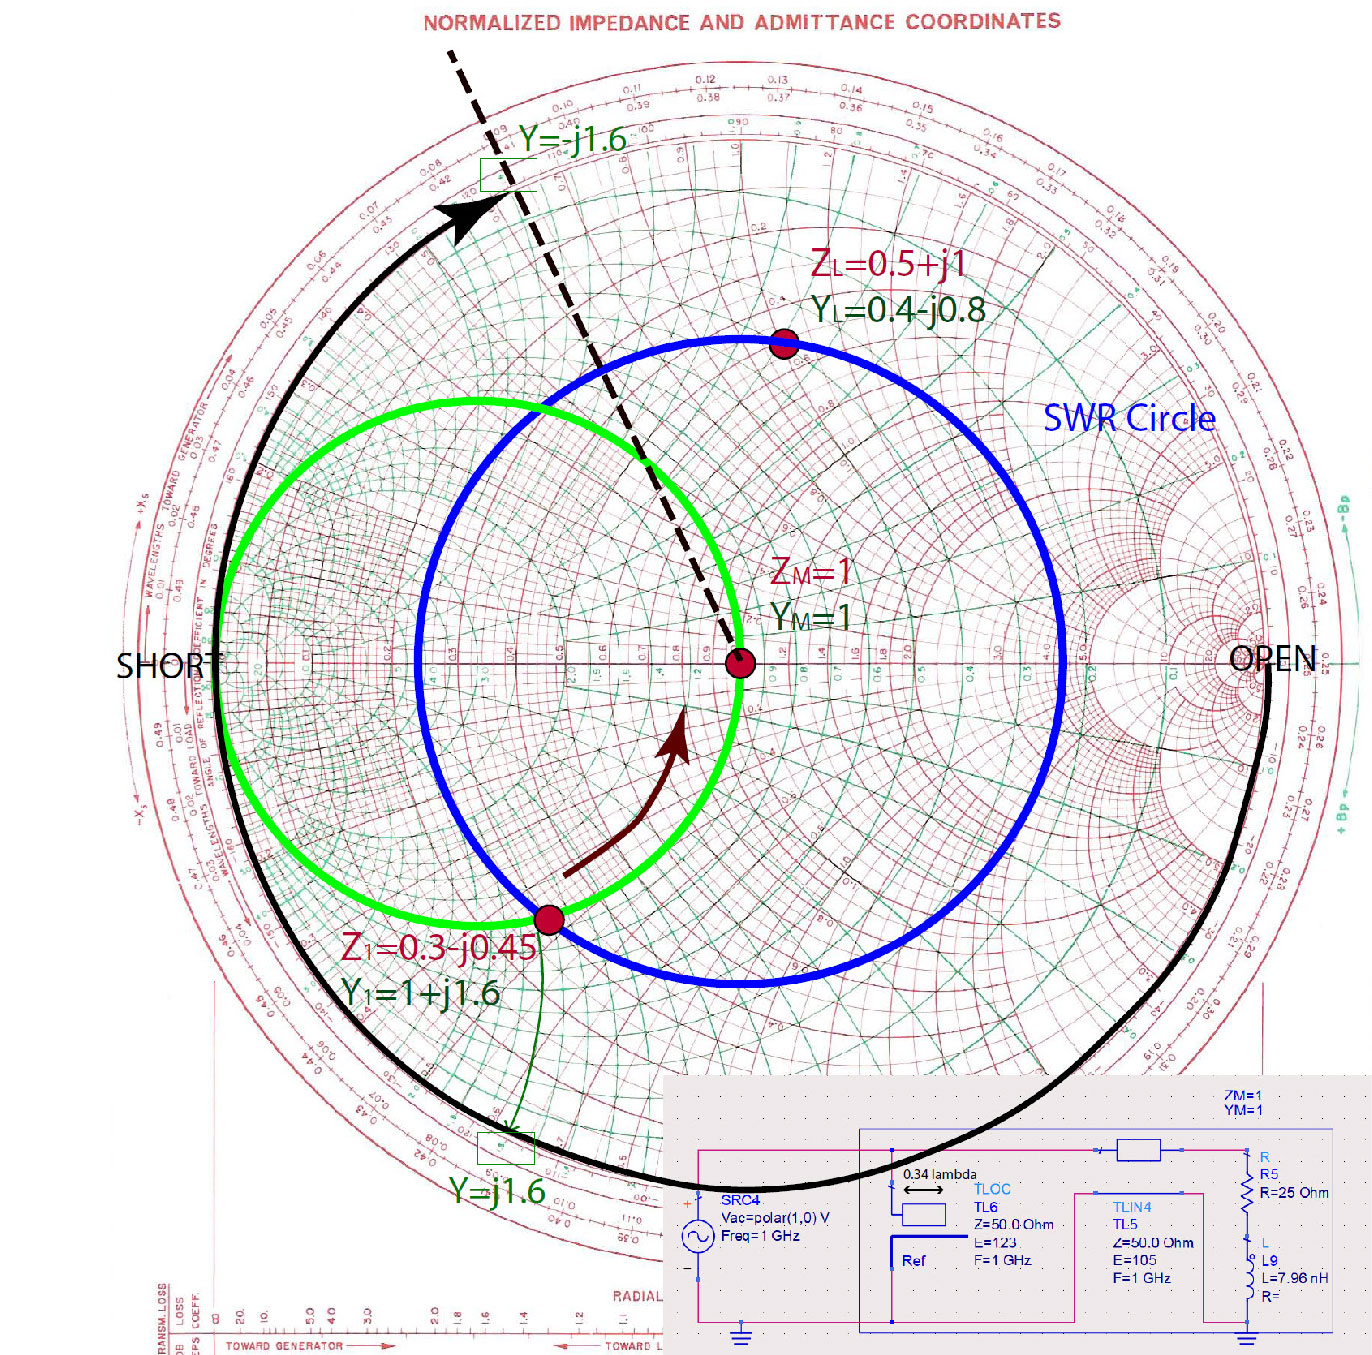
\includegraphics[scale=1]{../jpg/MatchTL-01.jpg}
\end{center}
\caption{Transmission-line impedance matching circuit.}
\label{fig:TransLineImpM}
\end{figure}

\end{document} 

